\chapter{Conditional Diffusion Models} \label{ch:conditional-diffusion}

So far we have described diffusion models as models that can be fit to describe a single distribution. In this chapter we introduce and motivate conditional diffusion models. A conditional diffusion model is trained on paired data $\rvx, \rvy \sim p_\text{data}(\cdot, \cdot)$ and then, at test-time, can be given $\rvy$ as an input and then produces samples from an approximation of the conditional distribution $p_\text{data}(\rvx|\rvy)$. Conditional diffusion models have applications in text-to-image systems (\cref{fig:dalle-3-samples}), image editing tools (\cref{fig:emu-edit-samples}), and more domains as we will describe in \cref{sec:conditional-diffusion-tasks}. Additionally, as we will discuss in \cref{sec:2sdm}, conditional diffusion models can often generate more realistic samples than unconditional diffusion models. Developing conditional diffusion models can therefore be useful even if the task of interest is to model a single distribution without conditioning. Before this, we will formally transport the important results of \cref{ch:diffusion} from the unconditional diffusion model setting to the conditional diffusion model setting in \cref{sec:conditional-diffusion-overview}.

\begin{figure}[t]
    \centering
    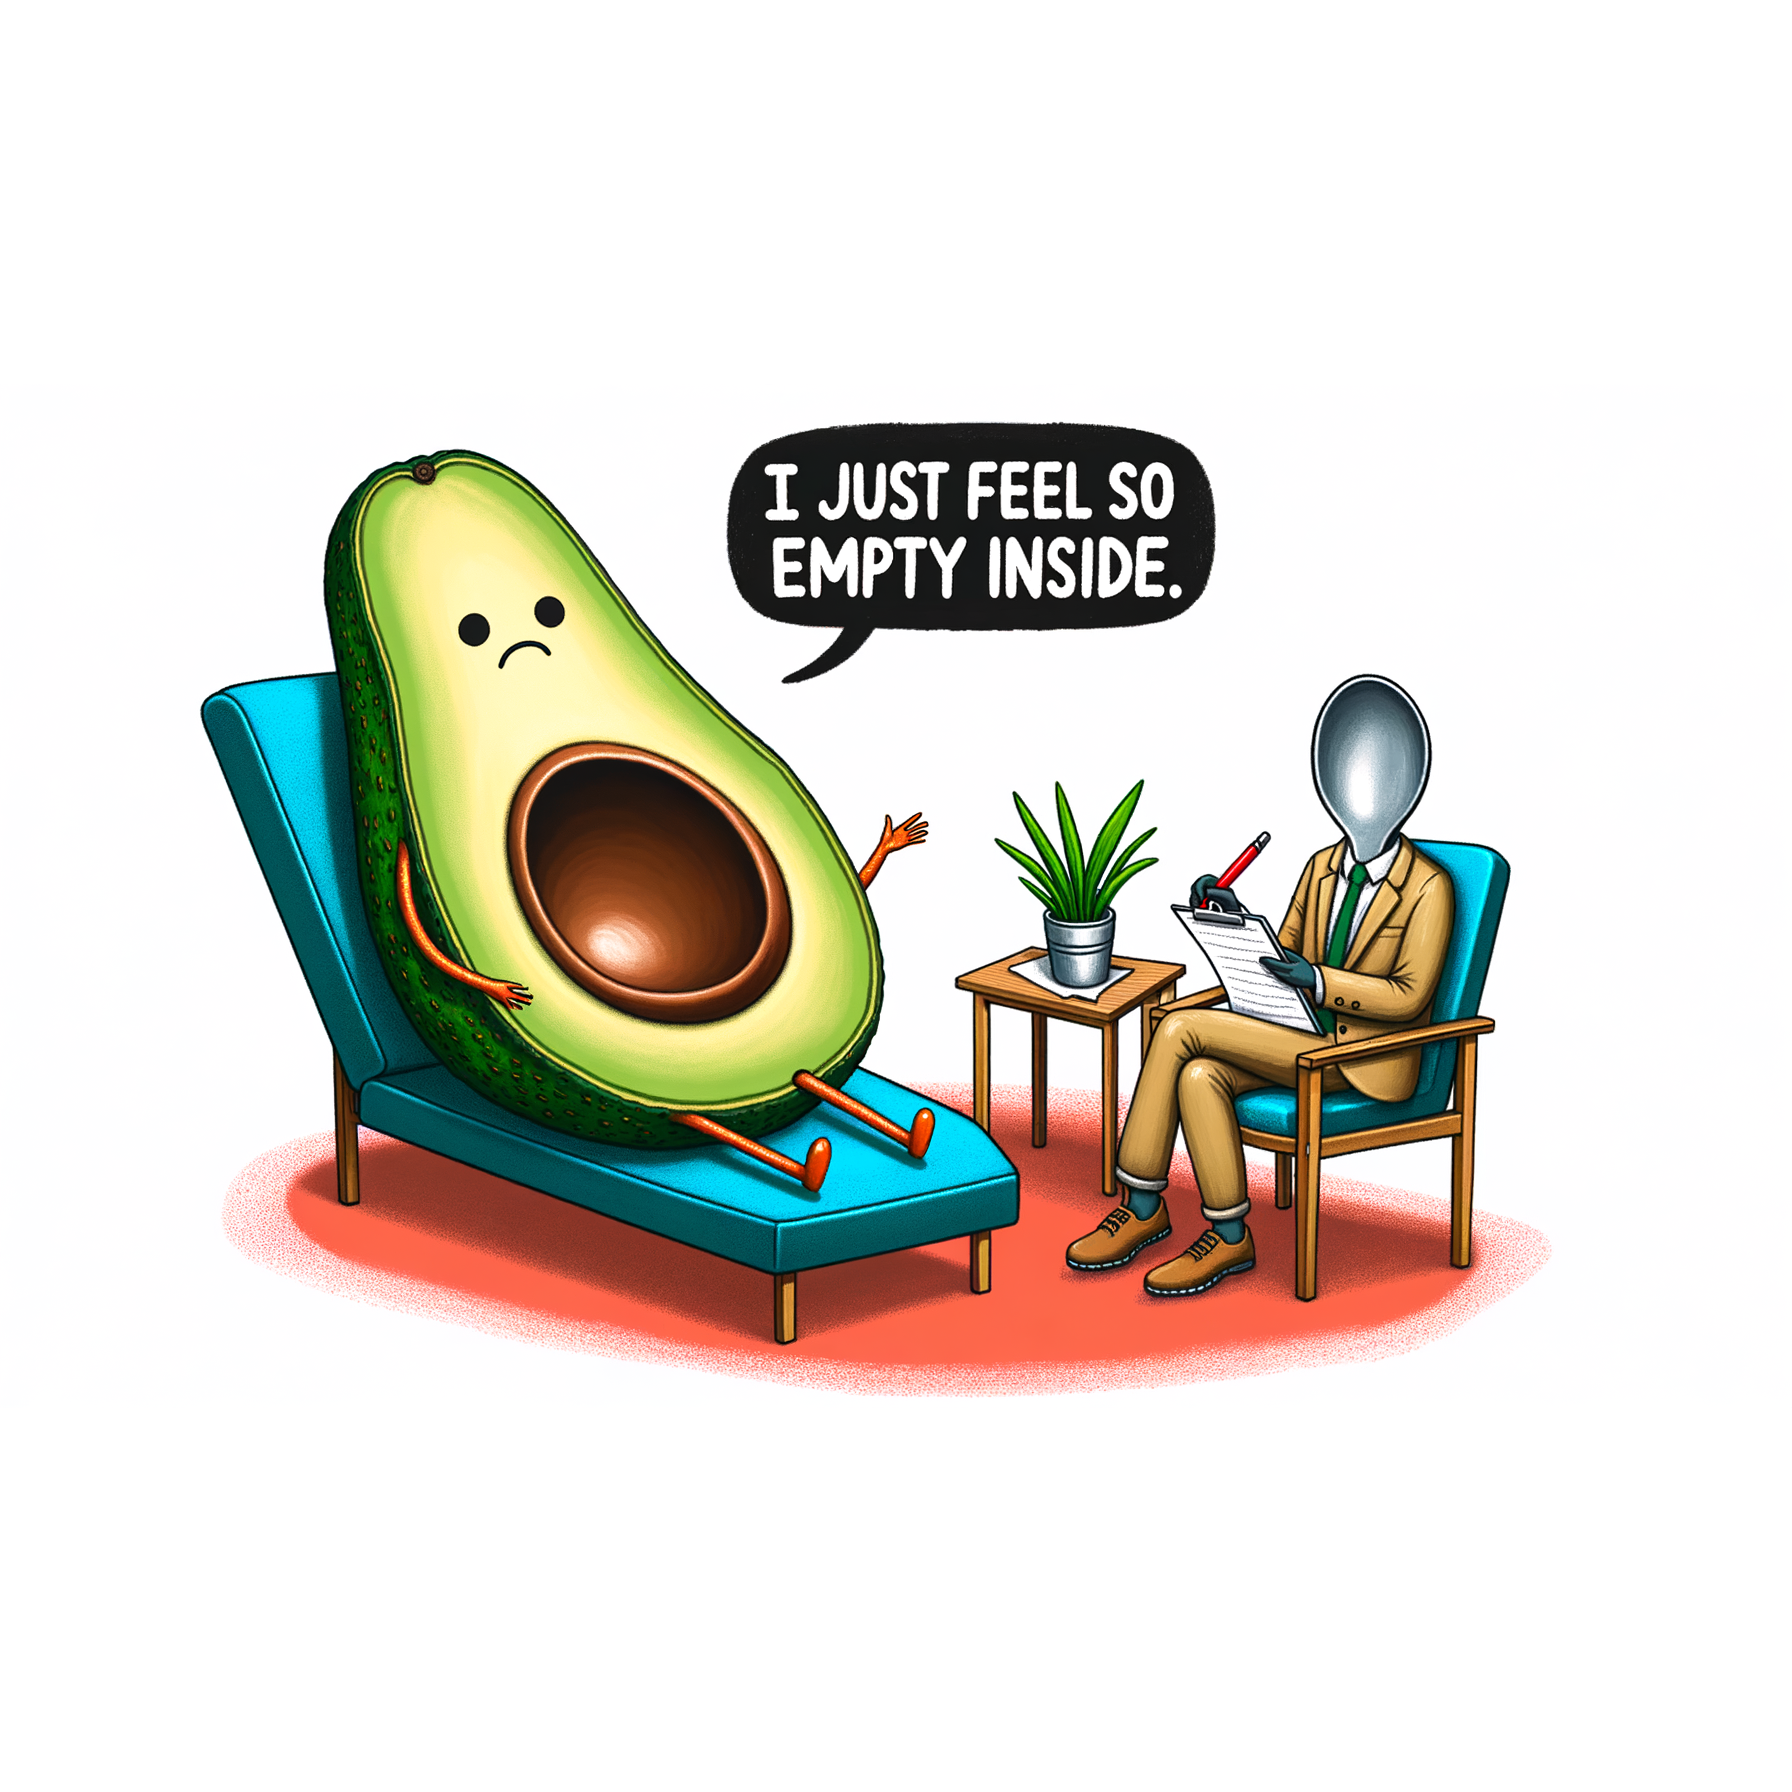
\includegraphics[width=0.32\textwidth]{figs/thesis/dalle3/1.png}
    \hfill
    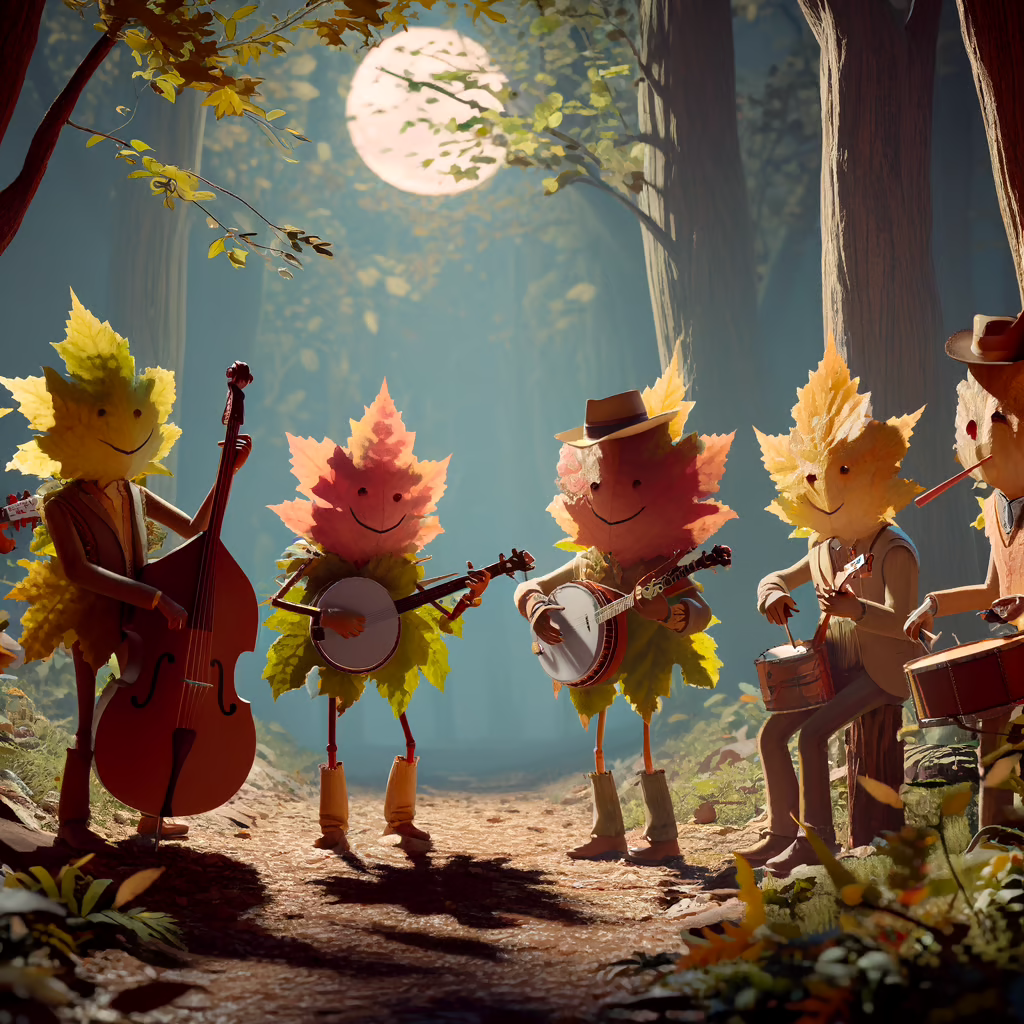
\includegraphics[width=0.32\textwidth]{figs/thesis/dalle3/2.png}
    \hfill
    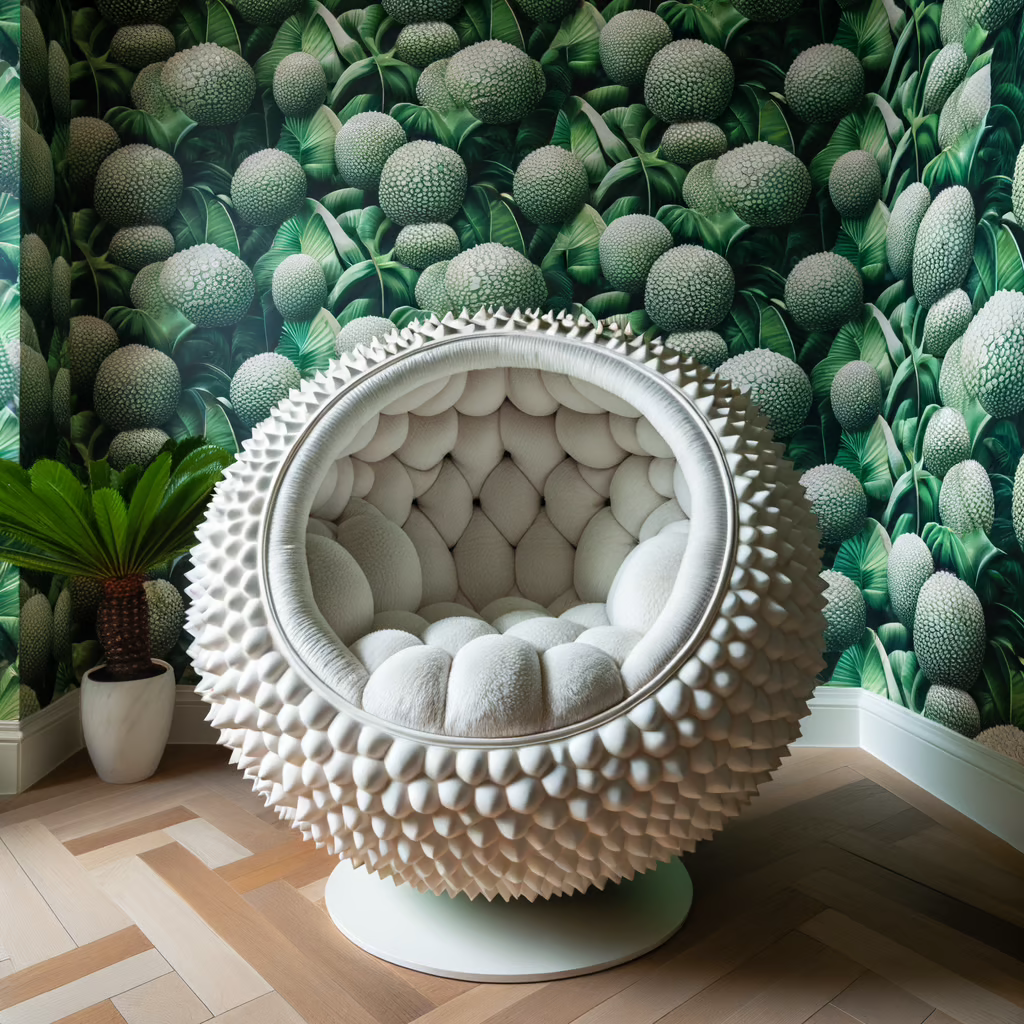
\includegraphics[width=0.32\textwidth]{figs/thesis/dalle3/4.png}
    \caption{Images sampled by DALL-E 3~\citep{betker2023improving} givne text prompts, from left to right, ``An illustration of an avocado sitting in a therapist's chair, saying 'I just feel so empty inside' with a pit-sized hole in its center. The therapist, a spoon, scribbles notes.''; ``A 2D animation of a folk music band composed of anthropomorphic autumn leaves, each playing traditional bluegrass instruments, amidst a rustic forest setting dappled with the soft light of a harvest moon.''; and ``Photo of a lychee-inspired spherical chair, with a bumpy white exterior and plush interior, set against a tropical wallpaper.''. Images reproduced from \citet{betker2023improving} (TODO permission).}
    \label{fig:dalle-3-samples}
    \centering
    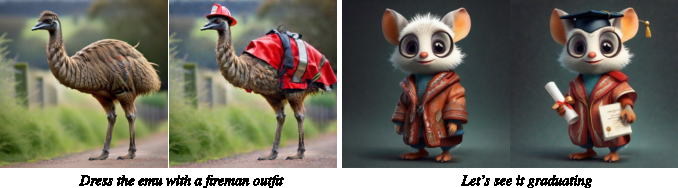
\includegraphics{figs/thesis/emu_edit_examples.pdf}
    \caption{Image-editing examples from Emu Edit~\citep{sheynin2023emu}, reproduced from \citet{sheynin2023emu} (TODO permission). Given an input image (left of each pair) and text prompt, Emu Edit samples an edited image (right of each pair).}
    \label{fig:emu-edit-samples}
\end{figure}

\section{Conditional Diffusion Modelling Overview} \label{sec:conditional-diffusion-overview}

In this section we will restate the main results from \cref{ch:diffusion} to be compatible with the conditional diffusion modelling setting. In this setting we will assume that there is a data distribution $p_\text{data}(\rvx, \rvy)$ and we can access samples from it to train our model. We will now call the distribution over $\rvx$ parameterised by our model $p_\theta(\rvx|\rvy)$ instead of $p_\theta(\rvx)$, and our objective is to match it to the conditional distribution $p_\text{data}(\rvx|\rvy)$. We will refer to $\rvy$ as the ``conditioning information''. It can take the form of, for example, an image, a text prompt, a class label, and embedding vector, or a combination of multiple such items.

Recall that the only part of the diffusion model that needed to be fit based on the target distribution (i.e. the dataset) in \cref{ch:diffusion} was the learned score function $\rvs_\theta(\rvx_\sigma, \sigma)$. If we want to model a family of distributions, i.e. $p_\text{data}(\rvx|\rvy)$ for various values of $\rvy$, all we then have to do is to learn a different score function for each distribution (i.e. for each value of $\rvy$). A simple way to achieve this is to feed $\rvy$ into the neural network as an additional input. Then we can view the neural network as parameterising a different mapping from $\rvx_t$ and $t$ to its output for any given value of $\rvy$. To make explicit the dependence on $\rvy$, we will call this conditional score function estimate $\rvs_\theta(\rvx_\sigma, \rvy, \sigma)$. We can use the same training and sampling procedures as in \cref{ch:diffusion}, as long as the appropriate value of $\rvy$ is fed in for each data point during training and the desired value of $\rvy$ is fed in at for each network evaluation during sampling. To support this high-level understanding, in the remainder of this section we will transport the most significant results from the previous chapter into the conditional diffusion setting.

Our forward SDE did not depend on any properties of the data or target distribution, and so it remains the same as in \cref{eq:forward-diffusion},
\begin{equation}
    \mathrm{d}\rvx = g(t) \mathrm{d}\rvw.
\end{equation}
We do not, at any point, add noise to the conditioning information $\rvy$. To simulate the reverse SDE, we now use our learned, $\rvy$-dependent, score function estimate so \cref{eq:reverse-diffusion-with-nn} becomes
\begin{align}
    \mathrm{d}\rvx = -g(t)^2 s_\theta(\rvx_t, \rvy, t) \mathrm{d}t + g(t) \mathrm{d}\bar{\rvw}.
\end{align}
Similarly, the dynamics of the reverse ODE in \cref{eq:reverse-diffusion-with-nn} become
\begin{align}
    \mathrm{d}\rvx = - \frac{1}{2} g(t)^2 s_\theta(\rvx_t, \rvy, t) \mathrm{d}t.
\end{align}

As in the unconditional setting, we can transform back and forth between an estimated score function, $s_\theta(\rvx_t, \rvy, t)$; an estimate of the original data which we call $\rvx_\theta(\rvx_t, \rvy, t)$; and an estimate of $\epsilon$ which we call $\mathbf{\epsilon}_\theta(\rvx_t, \rvy, t)$. For simplicity, in this section we will describe all losses in terms of the squared error in the prediction of $\rvx$. To design a loss that is good for a single $\rvy$, we can modify \cref{eq:diffusion-loss-all-sigma} to replace the unconditional distribution $\pdata(\rvx)$ with the desired conditional distribution $\pdata(\rvx|\rvy)$, and to give the neural network $\rvy$ as an additional input:
\begin{align} \label{eq:cond-diffusion-loss-non-amortized}
    \mathcal{L}_\text{ISM}(\theta; \rvy) &= \int_{\sigma_\text{min}}^{\sigma_\text{max}} \lambda^\rvx(\sigma) \EX_{q(\rvx, \rvx_\sigma|\rvy)} \left[ 
    || \rvx_\theta(\rvx_\sigma, \rvy, \sigma) - \rvx ||_2^2 \right] \mathrm{d}\sigma
\end{align}
where $q(\rvx, \rvx_\sigma|\rvy)$ is defined as $\pdata(\rvx|\rvy) q(\rvx_\sigma|\rvx)$. This may be difficult to sample from in practice if it is difficult to sample from $\pdata(\rvx|\rvy)$, which may be the case if for example we have a finite-sized dataset and few or no data points with the desired value of $\rvy$. Additionally, when training a conditional diffusion model, we would usually like the model to work well for many different values of the conditioning information $\rvy$. We can solve both of these problems by taking an expectation of \cref{eq:cond-diffusion-loss-non-amortized} over $\pdata(\rvy)$:
\begin{align} \label{eq:cond-diffusion-loss}
    \mathcal{L}_\text{ISM}(\theta) &= \EX_{\pdata(\rvy)} \left[ \int_{\sigma_\text{min}}^{\sigma_\text{max}} \lambda^\rvx(\sigma) \EX_{q(\rvx, \rvx_\sigma|\rvy)} \left[ 
    || \rvx_\theta(\rvx_\sigma, \rvy, \sigma) - \rvx ||_2^2 \right] \mathrm{d}\sigma \right] \\
    &= \int_{\sigma_\text{min}}^{\sigma_\text{max}} \lambda^\rvx(\sigma) \EX_{q(\rvx, \rvx_\sigma,\rvy)} \left[ 
    || \rvx_\theta(\rvx_\sigma, \rvy, \sigma) - \rvx ||_2^2 \right] \mathrm{d}\sigma 
\end{align}
where $q(\rvx, \rvx_\sigma,\rvy) = \pdata(\rvx,\rvy)q(\rvx_\sigma|\rvx)$. Now the difference between this loss and the unconditional diffusion model loss in \cref{eq:diffusion-loss-all-sigma} is just that we sample conditioning information $\rvy$ along with each piece of data to generate, $\rvx$, and feed it into the neural network as an extra input.

% We re-derive in the appendix the loss weighting $\lambda^\rvx(\sigma) = \frac{2}{\sigma^3}$ that makes the diffusion objective lower-bound the data likelihood, showing that it is the same in the conditional diffusion setting as in the unconditional setting.


\section{Conditional Generation Tasks} \label{sec:conditional-diffusion-tasks}

A primary reason to use conditional generative models is to enable conditional generation tasks. In the image domain, examples of these include inpainting, text-conditional generation, and image editing. Analogues of all of these exist in the video domain as well~\cite{ho2022imagen}. In this section we briefly touch on some other use cases for conditional diffusion models: as a world model or planner for an embodied agent; and as an alternative to a deterministic, hand-written algorithm for many types of computational problem.

\begin{figure}
    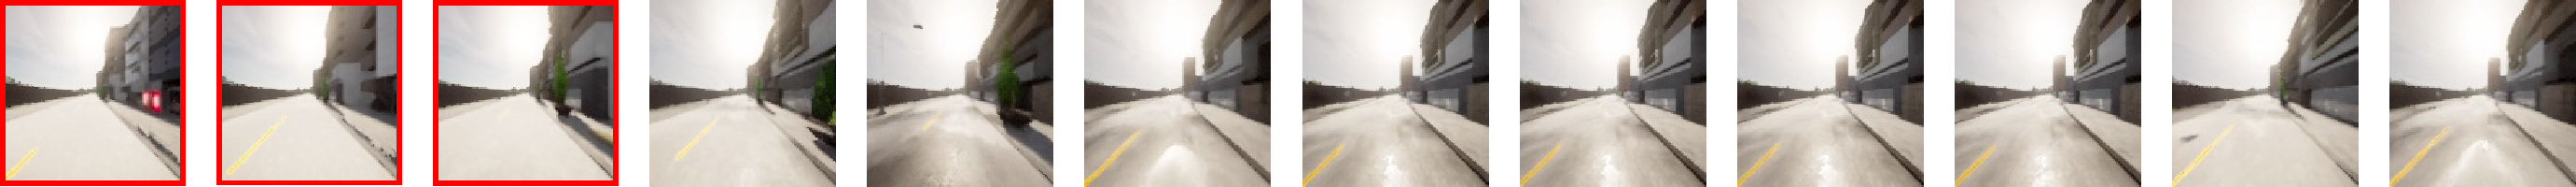
\includegraphics[width=\textwidth]{figs/thesis/fdm-example-tasks/world-modeling-thesis.pdf}
    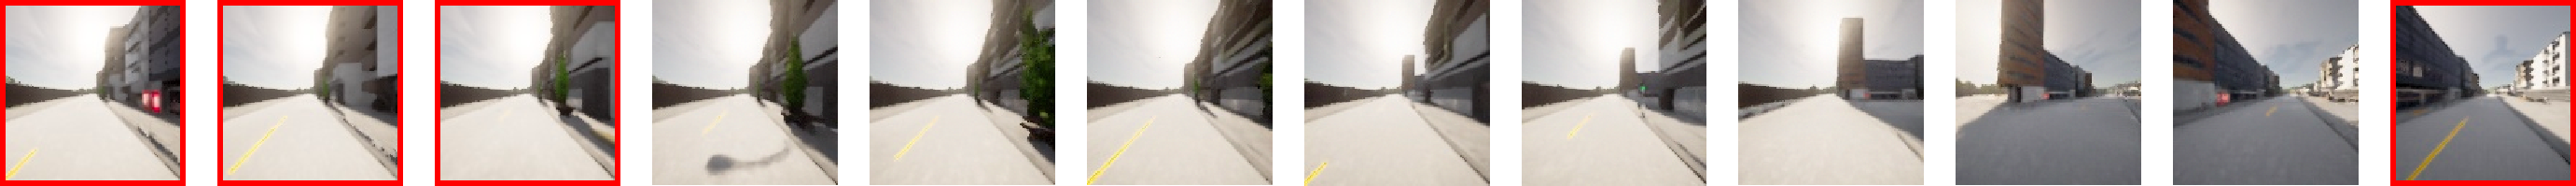
\includegraphics[width=\textwidth]{figs/thesis/fdm-example-tasks/visual-planning-thesis.pdf}
    \caption{Video generation tasks on a first-person view autonomous driving dataset solved by 
    the diffusion model introduced in \cref{ch:fdm}. \textbf{Top:} We condition on 3 frames, each 1 second apart, and predict the next 9 frames. In this way, we can use the model as a ``world model'' that predicts both the agent's actions and the environment dynamics. \textbf{Bottom:} We condition on both the first 3 frames and the final frame. The final frame serves as a description of the goal. The model now serves as a route planner: with the generated frames plotting a route from the current position, as summarised by the first three frames, to the desired position.}
    \label{fig:fdm-example-tasks}
\end{figure}

In \cref{fig:fdm-example-tasks} we show a conditional diffusion model being used a ``world model''. This conditional diffusion model, which we will describe in more detail in \cref{ch:fdm}, is trained on a dataset of videos generated from a first-person viewpoint of a simulated vehicle driving around a single virtual town. In the top row of \cref{fig:fdm-example-tasks}, we show the first three video frames (with red outlines) being fed into the model as the conditioning information $\rvy$. In a reinforcement learning sense, these can be understood as a summary of the ``current state'' of the simulated agent. We then use the conditional diffusion model to predict nine future frames. Inspecting the frames, the diffusion model models the agent as slowly moving forward, then coming upon a red traffic light and coming to a stop. Implicitly this conditional model must therefore contain both a world model, which models the appearance of the world as the agent moves forward and e.g. that the traffic light will be red, and an implicit policy for the agent, which captures that the agent will at first move forward but will stop when it comes to the red traffic light. In the second row of \cref{fig:fdm-example-tasks}, we see a different conditional generation task. Now, as well as being conditioned on the first three frames to summarise the current state, the agent is also conditioned on the final frame, which we can view as a specification of a ``goal'' for the agent. Given these frames, the conditional diffusion model produces eight frames in between. These can be interpreted as a ``plan'' for how to get from the current position to the goal. In this case, the plan is to go to the traffic light, turn right, and then drive a short distance further.

\begin{figure}
    \centering
    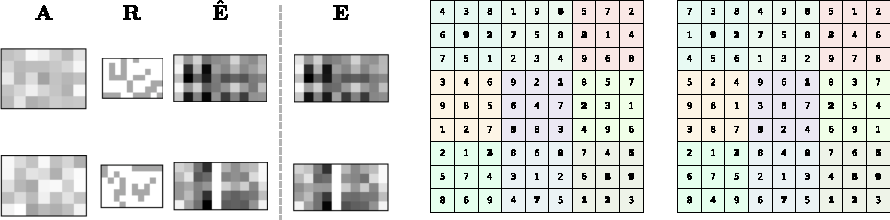
\includegraphics[width=\textwidth]{figs/thesis/gsdm-examples.pdf}
    \caption{
        \textbf{Left:} A matrix-factorisation problem. A diffusion model was used to sample $\rmA$ and $\rmR$ given $\rmE$ such that the product $\hat{\rmE} := \rmA \rmR$ is close to $\rmE$. \textbf{Right:} Solutions to a Sudoku puzzle sampled from a diffusion model. The given clues (bold) yield multiple solutions, and the two shown samples from the diffusion model are both valid.
    }
    \label{fig:gsdm-examples}
\end{figure}

The ``world modelling'' problem is inherently stochastic due to uncertain about the precise conditions in the world. We now argue that conditional diffusion models can also be the best approach for problems with no, or limited, stochasticity. \citet{weilbach2023graphically,weilbach2023scaling} demonstrate that conditional diffusion models outperform deterministic neural networks and other baselines for tasks including: Sudoku solving, in which there can be either one or more solutions (see \cref{fig:gsdm-examples}); matrix factorisation, where there are multiple solutions due to permutation invariances (see \cref{fig:gsdm-examples}); and sorting short lists, where there is a single solution. In these contexts, conditional diffusion models can be seen as swap-in replacements for a deterministic regressors that yield robustness to problems with multiple solutions.

In this section we have presented several use-cases for conditional diffusion models that would not make sense with unconditional diffusion models. In the next section, we make the case that there is one more advantage of conditional over unconditional diffusion models: empirically, samples generated by conditional diffusion models are often generate more realistic than those generated by unconditional diffusion models.

\section{Conditioning on More Information Improves Performance}

% \begin{figure}[t]
%     \centering
%     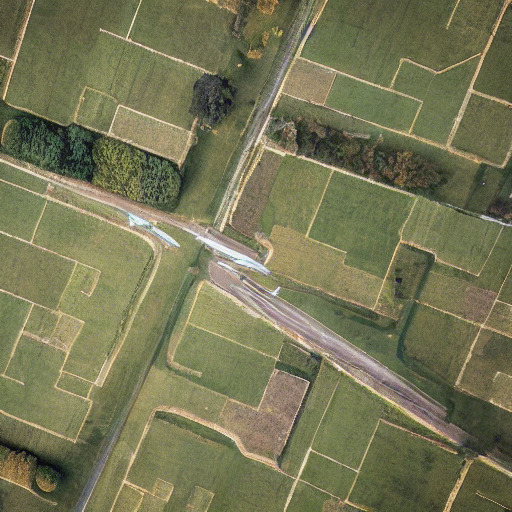
\includegraphics[width=0.24\textwidth]{figs/2sdm/uncond-aerial-photo.jpg}
%     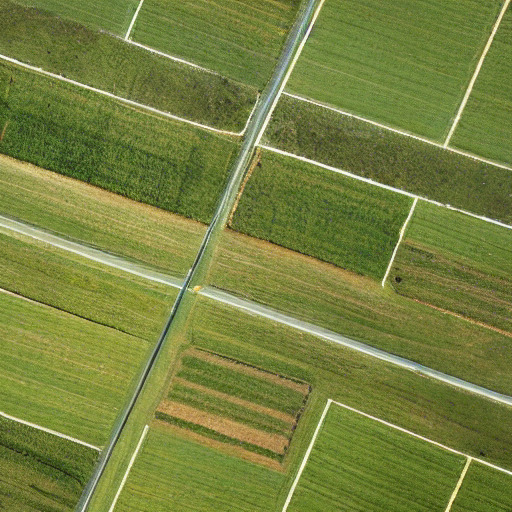
\includegraphics[width=0.24\textwidth]{figs/2sdm/cond-aerial-photo.jpg}
%     \caption{\textbf{Left:} Output from Stable Diffusion~\citep{rombach2022high} prompted to produce ``aerial photography''. \textbf{Right:} Using a more detailed prompt\protect\footnotemark with the same random seed removes the ``smudged'' road artifact that appears on the left. 2SDM builds on this observation.}
%     \label{fig:stable-diffusion-example}
% \end{figure}
\begin{figure}[t]
    \centering
    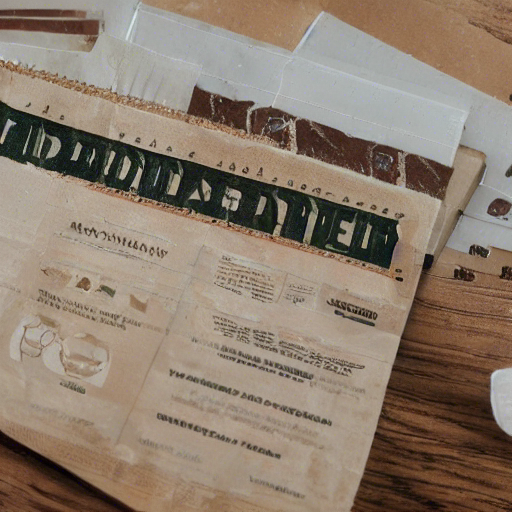
\includegraphics[width=0.3\textwidth]{figs/2sdm/sd_uncond.png}
    \hfill
    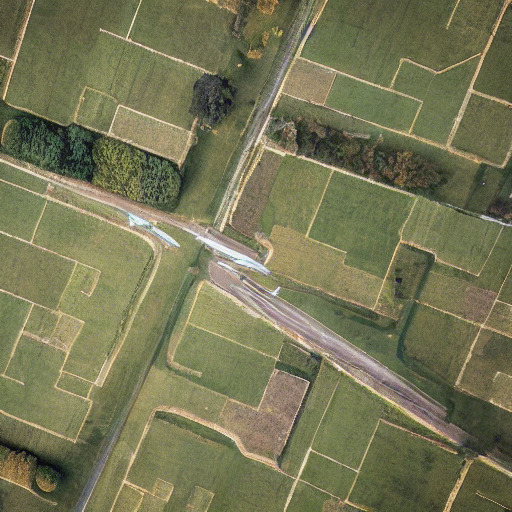
\includegraphics[width=0.3\textwidth]{figs/2sdm/uncond-aerial-photo.jpg}
    \hfill
    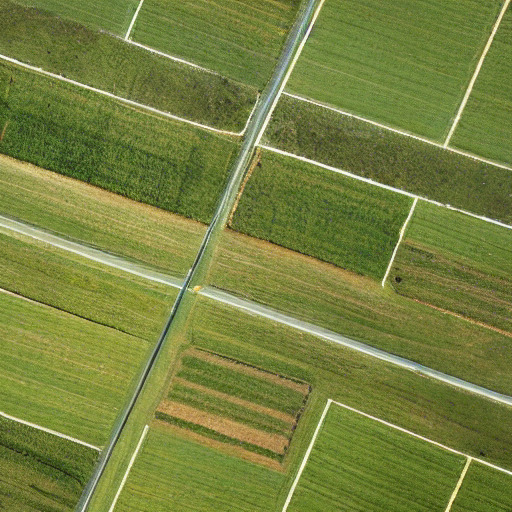
\includegraphics[width=0.3\textwidth]{figs/2sdm/cond-aerial-photo.jpg}
    \caption{Outputs from Stable Diffusion~\citep{rombach2022high} with the same random seed and three text prompts. \textbf{Left:} Output with an exmpty text prompt. \textbf{Middle:} Output when prompted to produce ``aerial photography''. \textbf{Right:} Output using a more detailed prompt\protect\footnotemark removes the ``smudged'' road artefact visible in the middle.}
    \label{fig:stable-diffusion-example}
\end{figure}
\footnotetext{We used the prompt ``Aerial photography of a patchwork of small green fields separated by brown dirt tracks between them. A large tarmac road passes through the scene from left to right.''}


% \label{sec:2sdm}
% We have introduced diffusion models as conditional generative models which take a conditioning input $\rvy$. In the remainder of this thesis, we will introduce innovations that will enable the same trained neural network to be conditioned on a wide range of different types of inputs $\rvy$. 

% Before that, in this chapter, we wish to motivate 

In this section we make the case that conditional diffusion models often achieve better sample quality than unconditional diffusion models. We will show that this insight can even be used to make improved \textit{unconditional} generative models that incorporate \textit{conditional} diffusion models.

% Prior work has shown that, if $\rvy$ is a text prompt, the resulting text-conditional diffusion models can have stunning sample quality and even be usable as artistic tools~\citep{saharia2022photorealistic,oppenlaender2022creativity}. Other effective types of conditional generation explored in prior work include conditioning on scene layouts~\citep{zhang2023adding}, segmentation masks~\citep{zhang2023adding,hu2022self}, or the appearance of a particular object \citep{ma2023unified}. We broadly lump these methods together as ``conditional'' DMs to contrast them with ``unconditional'' image DMs which sample an image without dependence on text or any other information. Unconditional image DMs fit into the framework described if $\rvy$ is considered to be the null variable, but we will usually omit $\rvy$ totally when describing them.

The better realism of samples from conditional DMs versus unconditional DMs has previously been noted by \citet{ho2022classifier,bao2022conditional,hu2022self}. Conditional DMs have also been observed to work better with few sampling steps~\citep{meng2022distillation}. Furthermore, we will show that sample realism grows with ``how much'' information the DM is conditioned on. To better make this point, we will distinguish between ``strongly-conditional'' generation, where we condition on a high-dimensional feature like a long text prompt, and ``lightly-conditional'' generation, where we condition on a lower dimensional feature like a class label or short text prompt.  As hinted at in \cref{fig:stable-diffusion-example} an image is likely to be more realistic if conditioned on being ``an aerial photograph of a road between green fields'' (strongly-conditional generation) than if it is if simply conditioned on being ``an aerial photograph'' (lightly-conditional generation). 

\subsection{Conditional vs unconditional DMs} \label{sec:2sdm-cond-vs-uncond-dgms}

We will investigate the phenomenon of conditional DMs outperforming unconditional DMs primarily in the context of conditioning on CLIP (contrastive language-image pre-training)~\citep{radford2021learning} image embeddings. These are embedding vectors encoding high-level, semantically-meaningful information about a given image. The training procedure for such an image embedder is as follows. CLIP jointly trains two neural networks, an image embedder $e_i(\cdot)$ and a text embedder $e_t(\cdot)$, trained on a large captioned-image dataset. Given an image $\rvx$ and a caption $\rvy$, the training objective encourages the cosine similarity between $e_i(\rvx)$ and $e_t(\rvy)$ to be large if $\rvx$ and $\rvy$ are a matching image-caption pair and small if not.
% The embedders are trained by separately embedding images and captions, and encouraging the cosine similarity between embeddings to be large if they are of matching image-caption pairs and small if not.
The image embedder therefore learns to map from an image to a semantically-meaningful embedding capturing any features that may be included in a caption. We use a CLIP image embedder with the ViT-B/32 architecture and weights released by \citet{radford2021learning}. We can visualize the information captured by the CLIP embedding by showing the distribution of images produced by our conditional DM given a single CLIP embedding; see \cref{fig:samples}.

\paragraph{What does it mean to say that conditional DMs beat unconditional DMs?} A standard procedure to evaluate unconditional DMs is to start by sampling a set of $N$ images independently from the model: ${\rvx^{(1)},\ldots,\rvx^{(N)} \sim p_\theta(\cdot)}$. We can then compute the Fr\'echet Inception distance (FID)~\citep{heusel2017gans} between this set and the dataset. If the generative model matches the data distribution well, the FID will be low.
%
For conditional DMs the standard procedure has one extra step: we first independently sample ${\rvy^{(1)},\ldots,\rvy^{(N)} \sim \pdata(\cdot)}$. We then sample each image given the corresponding $\rvy^{(i)}$ as ${\rvx^{(i)} \sim p_\theta(\cdot|\rvy^{(i)})}$. 
%
Then, as in the unconditional case, we compute the FID between the set of images $\rvx_1,\ldots,\rvx_N$ and the dataset, without reference to $\rvy_1,\ldots,\rvy_N$. Even though it does not measure alignment between $\rvx, \rvy$ pairs, conditional DMs beat comparable unconditional DMs on this metric in many settings: class-conditional CIFAR-10 generation~\citep{karras2022elucidating}, segmentation-conditional generation~\citep{hu2022self}, or bounding box-conditional generation~\citep{hu2022self}.

\begin{figure}[t]
    \centering
    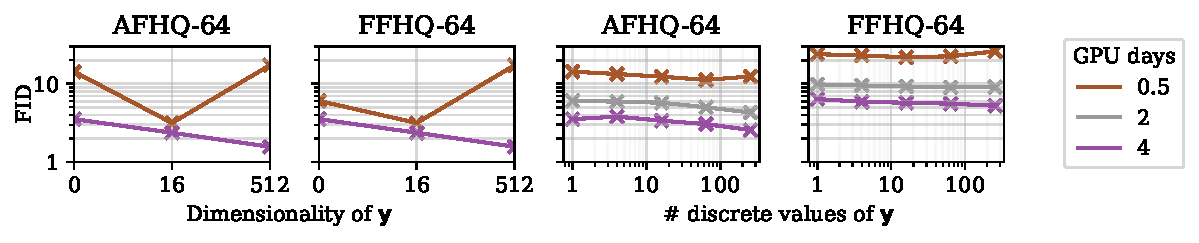
\includegraphics[width=\textwidth]{figs/2sdm/cond-results-vs-nclusters.pdf}
    \caption{FID versus dimensionality of $\rvy$ on AFHQ~\citep{choi2020stargan} and FFHQ~\citep{karras2018style}. With small training budgets (brown line), it is harmful when $\rvy$ is too informative. With larger training budgets (purple line), it is helpful to make $\rvy$ much more high dimensional.}
    \label{fig:fid-vs-ncomp}
\end{figure}

\paragraph{Why do conditional DMs beat unconditional DMs?}

Conditional DMS ``see'' more data during training than their unconditional counterparts because updates involve $\rvy$ as well as $\rvx$. \citet{bao2022conditional,hu2022self} prove that this is not the sole reason for their successes because the effect holds up even when $\rvy$ is derived from an unconditional dataset through self-supervised learning.
%
To our knowledge, the best explanation for their success is, as stated by \citet{bao2022conditional}, that conditional distributions typically have ``fewer modes and [are] easier to fit than the original data distribution.''

\paragraph{When do conditional DMs beat unconditional DMS?}
%
We present results in \cref{fig:fid-vs-ncomp} to answer this question. We show FID scores for conditional DMs trained to condition on embeddings of varying information content. 
%
We produce $\rvy$ by starting from the CLIP embedding of each image in our dataset and using either principal component analysis to reduce their dimensionality (left two panels) or K-means clustering to discretize them (right two panels)~\citep{hu2022self}.
%
We see that, given a small training budget, it is best to condition on little information. With a larger training budget, performance appears to improve steadily as the dimensionality of $\mathbf{y}$ is expanded. We hypothesize that \textbf{(1)} conditioning on higher-dimensional $\mathbf{y}$ slows down training because it means that points close to any given value of $\mathbf{y}$ will be seen less frequently and $\textbf{(2)}$ with a large enough compute budget, any $\mathbf{y}$ correlated with $\mathbf{x}$ will be useful to condition on. This suggests that, as compute budgets grow, making unconditional DM performance match conditional DM performance will be increasingly useful.




\subsection{Using conditional DMs for unconditional tasks} \label{sec:2sdm-2sdm-method}

The gap in performance between conditional and unconditional DMs is problematic. Imagine you need to sample a dataset of synthetic aerial photos.\footnote{ This may be done to, e.g., later train state-of-the-art a classification system~\citep{azizi2023synthetic}.}. A researcher doing so would currently have to either (a) make up a scene description before generating each dataset image, and ensure these cover the entirety of the desired distribution, or (b) accept the inferior image quality gleaned by conditioning just on each image being ``an aerial photograph''.  \Cref{fig:stable-diffusion-example} shows that the difference in quality can be stark.

\begin{figure}[t]
    \centering
    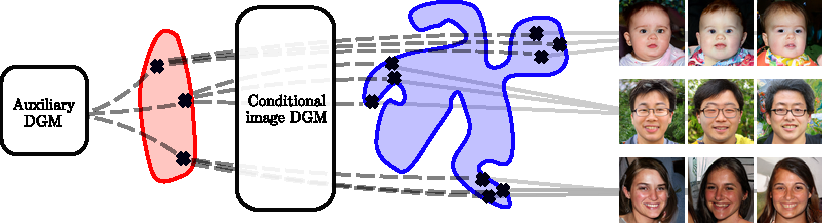
\includegraphics[width=\textwidth]{figs/2sdm/vcdm-diagram.pdf}
    \caption{Visualisation of 2SDM's generation process. First the auxiliary DM samples a CLIP embedding, corresponding to a cross in the space of CLIP embeddings (red) in our illustration. Next, our conditional image model maps from the sampled CLIP embedding to a sampled image, visualized on the image manifold (blue). The distribution over plausible images is complex and multi-modal but becomes simpler when conditioned on a CLIP embedding. On the right we show three rows of sampled images. Within each row, all images are generated given the same CLIP embedding.}
    \label{fig:samples}
\end{figure}

We therefore suggest a solution to this problem that comes from revisiting the methodology of DALL-E 2, also known as unCLIP~\citep{ramesh2022hierarchical}. UnCLIP is a method for text-conditional image generation which we describe in detail in \cref{sec:2sdm-background}. It was originally proposed as a way to ``invert'' a pretrained CLIP embedder and thereby map from text to image space but, perhaps due to improved text embeddings and a desire for methodological simplicity, we are not aware of future work building on the two-stage unCLIP approach~\citep{rombach2022high,chang2023muse,hoogeboom2023simple}. We hope to counter this trend, arguing that, while unCLIP may provide little benefit for ``strongly-conditional'' text-to-image generation (especially when the text prompt is long or heavily ``prompt-engineered''), its benefits are in fact much greater than previously acknowledged when applied to unconditional or ``lightly-conditional'' generation.

Our final approach, based on unCLIP, is depicted in \cref{fig:samples}. A first ``auxiliary DM'' samples vectors within an embedding space, with any vector describing a particular set of semantic characteristics of an image. The second stage, a ``conditional image DM'', takes such a vector as input and samples an image with these semantic characteristics. The vector embedding is informative, as evidenced by the fact that all images within each row on the right of \cref{fig:samples}, which are all conditioned on the same embedding, look very similar. The conditional image DM therefore inherits all the previously-described advantages of strongly-conditional DMs even though our overall generative model is unconditional (or, with the generalization we will introduce shortly, lightly-conditional). We call the resulting model a Two-Stage Diffusion Model (2SDM). We will now describe the form that these two models take in the experiments that we run with this architecture.

We will now introduce our notation for 2SDM. Recall that, for unconditional generation, the user does not wish to specify any input to condition on and, for the lightly-conditional setting, any such input is low-dimensional. This conditioning information is similar to the variable we have been calling $\rvy$ but, to distinguish it from the input to the conditional diffusion model itself, we will call it $\rva$ in both cases. Specifically, $\rva$ is a low-dimensional input in the lightly-conditional setting or a null variable in the unconditional setting. For the rest of this chapter we will use $\rvy := e_i(\rvx)$ to refer to a CLIP image embedding. To make this deterministic encoding compatible with a probabilistic generative modeling perspective, we consider a joint distribution $\pdata(\rvx, \rvy, \rva)=\pdata(\rvx, \rva)\delta_{e_i(\rvx)}(\rvy)$, where $\pdata(\rvx, \rva)$ is described by a dataset and $\delta_{e_i(\rvx)}(\rvy)$ is a Dirac conditional distribution enforcing that $\rvy$ is the CLIP embedding of $\rvx$. For the rest of this chapter all distributions denoted with $\pdata$ should be understood as marginals and/or conditionals of this joint distribution, including our target distribution $\pdata(\rvx|\rva)$. 2SDM approximates this target distribution as
%
\begin{align} \label{eq:no-a}
    \pdata(\rvx|\rva) &= \mathbb{E}_{\pdata(\rvy|\rva)} \left[ \pdata(\rvx|\rvy,\rva) \right] \\
    &\approx \mathbb{E}_{p_\phi(\rvy|\rva)} \left[ p_\theta(\rvx|\rvy,\rva) \right] % = p_{\theta,\phi}(\rvx|\rva)
\end{align}
where $p_\phi(\rvy|\rva)$ is a second DM modeling the CLIP embeddings. We can sample from this distribution by sampling $\rvy\sim p_\phi(\cdot|\rva)$ and then leveraging the conditional image DM to sample $\rvx \sim p_\theta(\cdot|\rvy,\rva)$ We then return $\rvx$ and make no further use of $\rvy$.
%
From now on we will call $p_\theta(\rvx|\rvy,\rva)$ the \textit{conditional image model} and $p_\phi(\rvy|\rva)$ the \textit{auxiliary model}. In our experiments the auxiliary model uses a small architecture relative to the conditional image model and so adds little extra cost.\footnote{For our ImageNet experiments, sampling from our auxiliary model takes 35ms per batch item. Sampling from our image model takes 862ms and so 2SDM has inference time only $4\%$ greater than our baselines.}


\paragraph{Auxiliary model}
Our auxiliary model is a conditional DM targeting $\pdata(\rvy|\rva)$, where $\rvy$ is a 512-dimensional CLIP embedding. Following \cref{eq:diffusion-loss}, we train it by minimizing
\begin{equation}
\label{eq:auxiliary-model-objective}
    \mathbb{E}_{u(\sigma)p_\sigma(\rvy_\sigma|\rvy,\sigma)\pdata(\rvy,\rva)} \left[ \lambda(\sigma) \lvert\lvert \rvy - \hat{\rvy}_\theta(\rvy_\sigma, \rva, \sigma) \rvert\rvert^2 \right].
\end{equation}
Analogously to \cref{eq:diffusion-loss}, $\rvy_\sigma \sim p_\sigma(\cdot|\rvy,\sigma)$ is a copy of the CLIP embedding $\rvy$ corrupted with Gaussian noise, and $u$ and $\rvy$ are the training distribution over noise standard deviations and weighting function respectively.
We follow the architectural choice of \citet{ramesh2022hierarchical} and use a DM with a transformer architecture. It takes as input a series of 512-dimensional input tokens: an embedding of $\sigma$; an embedding of $\rva$ if this is not null; an embedding of $\rvy_\sigma$; and a learned query. These are passed through six transformer layers and then the output corresponding to the learned query token is used as the output. Like \citet{ramesh2022hierarchical}, we parameterize the DM to output an estimate of the denoised $\rva$ instead of estimating the added noise as is more common in the diffusion literature.
%
On AFHQ and FFHQ we find that data augmentation is helpful to prevent the auxiliary model overfitting. We perform augmentations (including rotation, flipping and color jitter) in image space and feed the augmented image through $e_i(\cdot)$ to obtain an augmented CLIP embedding. Following \citet{karras2022elucidating}, we pass a label describing the augmentation into the transformer as an additional input token so that we can condition on there being no augmentation at test-time.

\begin{figure}[t]
    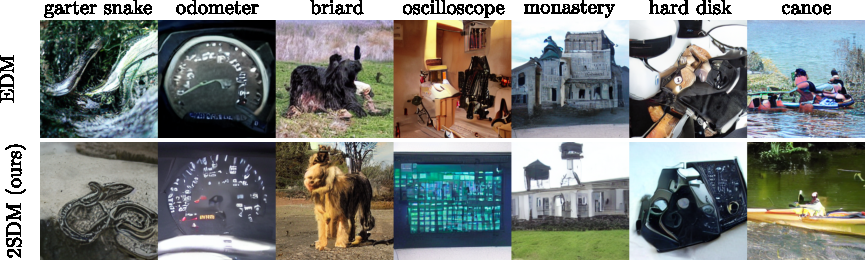
\includegraphics[width=\textwidth]{figs/2sdm/2SDM-main-fig.pdf}
    \caption{Class-conditional ImageNet-256 samples from our method, 2SDM, and a diffusion model baseline, EDM~\citep{karras2022elucidating}, both trained for 12 GPU days. Samples within the same column are generated with the same random seed and class label. In most columns the samples from 2SDM are visibly better, agreeing with the FIDs reported in \cref{sec:2sdm-experiments}.}
    \label{fig:latent-imagenet-samples}
\end{figure}

\paragraph{Conditional image model}
Including the additional conditioning input $\rva$, the conditional image model's training objective is
\begin{equation}
\label{eq:conditional-image-model-objective}
    \mathbb{E}_{u(\sigma)p_\sigma(\rvx_\sigma|\rvx,\sigma)\pdata(\rvx,\rvy,\rva)} \left[ \lambda(\sigma) \lvert\lvert \rvx - \hat{\rvx}_\theta(\rvx_\sigma, \rvy \oplus \rva, \sigma) \rvert\rvert^2 \right].
\end{equation}
where $\rvy \oplus \rva$ is the concatenation of $\rvy$ and $\rva$ to form a single vector which the image model is conditioned on. We match our diffusion process hyperparameters, including $u$ and $\lambda$, to those of \citet{karras2022elucidating}, and also use their proposed Heun sampler.  For AFHQ and FFHQ, we use the U-Net architecture originally proposed by \citet{song2020score}. For ImageNet, we use the slightly larger U-Net architecture proposed by \citet{dhariwal2021diffusion}. We match the data augmentation scheme to be the same as that of \citet{karras2022elucidating} on each dataset. There are established conditional variants of both architectures~\citep{dhariwal2021diffusion,karras2022elucidating} that add a learned linear projection to the embedding of the noise standard deviation $\sigma$.  We use the same technique to incorporate the concatenated conditioning inputs $\rvy\oplus\rva$.

\begin{figure*}[t]
    \centering
    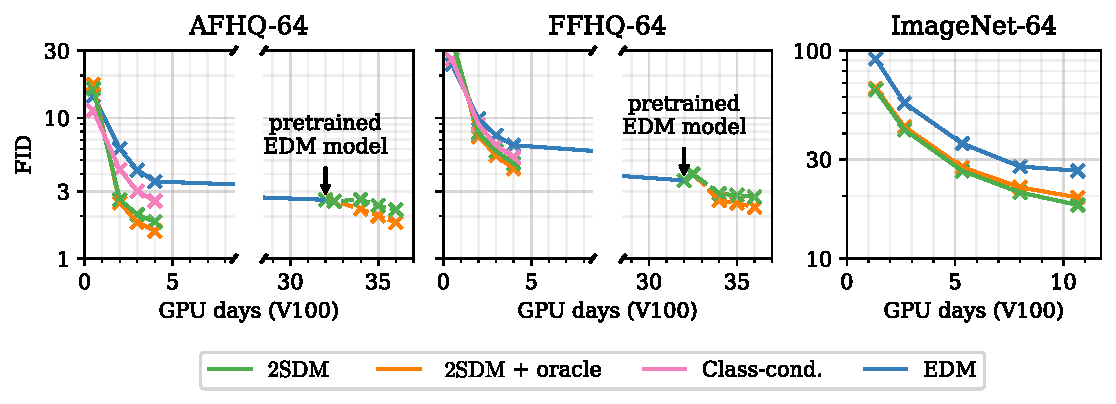
\includegraphics[width=\textwidth]{figs/2sdm/cond-results-1.pdf}
    \caption{FID throughout training. We show results for each method trained from scratch and, on AFHQ and FFHQ, for finetuning a pretrained EDM model (which was trained for the equivalent of 32 GPU days). 2SDM quickly outperforms EDM when trained from scratch and quickly improves on the pretrained model when used for finetuning.}
    \label{fig:fid_vs_training}
\end{figure*}

\subsection{2SDM improves over standard diffusion models} \label{sec:2sdm-experiments}


\begin{table}[t]
\centering
\caption{Comparison of 2SDM and EDM on a suite of metrics. Best performance for each metric and dataset is shown in bold. Higher is better for metrics marked $\uparrow$; lower is better for $\downarrow$. Results reported for EDM on FFHQ and AFHQ are computed with the pretrained checkpoints released by \citet{karras2022elucidating}. Results reported for 2SDM on FFHQ are with finetuning from this pretrained checkpoint. All others are trained from scratch.}
\begin{tabular}{lcccccccccc}
\toprule
 \multirow{2}{*}{Dataset} & \multirow{2}{*}{Method} & \multirow{2}{*}{\shortstack{Inception\\Score $\uparrow$}} & \multirow{2}{*}{Precision $\uparrow$} & \multirow{2}{*}{Recall $\uparrow$} & \multirow{2}{*}{FID $\downarrow$} & \multirow{2}{*}{sFID $\downarrow$} \\
 & & & & & & \\
\midrule
\multirow{2}{*}{AFHQ-64} & 2SDM & $\mathbf{10.00}$ & $\mathbf{0.844}$ & $\mathbf{0.619}$ & $\mathbf{1.56}$ & $13.7$ \\
 & EDM & $8.91$ & $0.752$ & $0.614$ & $2.04$ & $13.7$ \\
\midrule
\multirow{2}{*}{FFHQ-64} & 2SDM & $\mathbf{3.47}$ & $\mathbf{0.721}$ & $\mathbf{0.697}$ & $\mathbf{2.32}$ & $4.98$ & \\
 & EDM & $3.33$ & $0.697$ & $0.569$ & $2.46$ & $\mathbf{4.90}$ \\
\midrule
\multirow{2}{*}{\shortstack[l]{Class-cond. \\ ImageNet-64}} & 2SDM & $\mathbf{17.3}$ & $\mathbf{0.541}$ & $\mathbf{0.573}$ & $\mathbf{17.4}$ & $\mathbf{4.63}$ \\
 & EDM & $13.6$ & $0.530$ & $0.532$ & $25.4$ & $6.50$ \\
\midrule
\multirow{2}{*}{\shortstack[l]{Uncond. \\ ImageNet-64}} & 2SDM & $\mathbf{15.6}$ & $\mathbf{0.614}$ & $\mathbf{0.526}$ & $\mathbf{21.0}$ & $\mathbf{5.59}$ \\
 & EDM & $11.3$ & $0.523$ & $0.524$ & $35.1$ & $9.14$ \\
 \midrule
\multirow{2}{*}{\shortstack[l]{Class-cond. \\ latent \\ ImageNet-256}} & 2SDM & $\mathbf{52.1}$ & $\mathbf{0.590}$ & $0.603$ & $\mathbf{24.3}$ & $\mathbf{7.36}$ \\
 & EDM & $40.4$ & $0.532$ & $\mathbf{0.610}$ & $34.2$ & $9.59$ \\
\end{tabular}
\label{tab:2sdm-many-metrics}
\end{table}

\paragraph{Experimental setup and results overview}
%\begin{table}
We perform experiments in five settings: unconditional AFHQ modeling at $64\times64$ resolution~\citep{choi2020stargan}; unconditional FFHQ modeling at $64\times64$ resolution~\citep{karras2018style}; unconditional ImageNet modeling at $64\times64$ resolution~\citep{deng2009imagenet}; class-conditional ImageNet modeling at $64\times64$ resolution; and finally class-conditional latent ImageNet modeling at $256\times256$ resolution, in which we train the diffusion models in the latent space of the pretrained VAE used by Stable Diffusion~\citep{rombach2022high}. In every setting, we compare against EDM~\citep{karras2022elucidating}, a standard DM directly modeling $\pdata(\rvx|\rva)$, with an identical architecture to 2SDM. We match the training compute of our conditional image model with that of EDM in every case. The auxiliary model is trained for one day on a single V100 GPU so adds little additional cost. On AFHQ and FFHQ, we match the EDM parameters to those of \citet{karras2022elucidating}. On ImageNet-64, we have a smaller training budget and so decrease the batch size to 128 and the learning rate to $1\times10^{-4}$. For simplicity we match 2SDM to use the same learning rate and batch size.

For the first three of our listed settings, \cref{fig:fid_vs_training} reports the FID throughout the training of the conditional image diffusion model (or image DM baseline).\footnote{Each FID in \cref{fig:fid_vs_training} is estimated using $20\,000$ images, each sampled with the SDE solver proposed by \citet{karras2022elucidating} using 40 steps, $S_\text{churn}=50$, $S_\text{noise}=1.007$, and other parameters set to their default values. Our other reported FID scores use $50\,000$ samples, as is standard, and the same sampler hyperparameters.}  In each case, the auxiliary model is trained for one day on one V100 GPU. We consider training the conditional image model from scratch (for up to 4 GPU days on AFHQ and FFHQ, or up to 11 GPU days on ImageNet-64), and see that it improves upon our EDM baseline for any training budgets over 1-2 GPU days. For AFHQ, this improvement is so substantial that 2SDM's FID after two GPU days is better than that of the pretrained EDM model released by \citet{karras2022elucidating}, which was trained for the equivalent of 32 V100 GPU days. In addition to training from scratch, on AFHQ and FFHQ we consider initializing 2SDM's training from the pretrained EDM checkpoints. To do so, we simply add a learnable linear projection of the CLIP embedding and initialize its weights to zero. We see that this allows for a fast and significant improvement in FID over the baseline in each case. We note, though, that training 2SDM from scratch for 4 GPU days 
\begin{wraptable}{r}{0.6\textwidth}
%\vspace{-.4cm}
\centering
\caption{A comparison of FID with the state-of-the-art (SOTA) in bold. EDM (single seed) is our re-computation of the EDM's reported results using a single seed instead of taking the best of three.}
\label{tab:2sdm-sota}
\begin{tabular}{lccc}
\midrule
Dataset         & AFHQ-64 & FFHQ-64 \\
\midrule
PFGM++~\citep{xu2023pfgm++}          & $-$ & $2.43$ \\
EDM~\citep{karras2022elucidating}
& $1.96$ & $2.39$  \\
EDM (single seed)     & $2.04$ & $2.46$  \\
EDM-G++~\citep{kim2022refining}               & $-$    & $\mathbf{1.77}$  \\
2SDM            & $\mathbf{1.56}$ & $2.31$ \\
% \hline
% \textit{Overfit 2SDM}    & $\mathit{1.16}$ & $\mathit{3.33}$ \\
\end{tabular}
%\end{table}
\end{wraptable}
outperforms 4 GPU days of finetuning on AFHQ and so recommend training 2SDM from scratch when sufficient compute is available.

\Cref{fig:fid-vs-ncomp} also compares against ``2SDM + oracle'', which is a supposed upper bound on 2SDM's performance given by sampling a CLIP image embedding from an oracle (in practice, the dataset) and then using 2SDM's conditional image model to sample an image conditioned on it. It therefore describes the performance that 2SDM would achieve with a perfect auxiliary model. On AFHQ-64, 2SDM with an oracle achieves a FID $56\%$ lower than EDM. Without an oracle, 2SDM still achieves a FID $48\%$ lower than 2SDM. We therefore say that 2SDM yields an improvement $87\%$ as large as can be gleaned by using a purely conditional DM. Similarly for FFHQ, 2SDM obtains an improvement $81\%$ as large as is possible with a purely conditional DM.\footnote{See \cref{tab:2sdm-results-breakdown} for the FIDs used in these calculations.} We can therefore say that our cheaply-trained auxiliary model is good enough to allow us to capture the majority of the benefits of conditional generation for the unconditional generation task. Intriguingly,
 on ImageNet-64, 2SDM achieves better FID \textit{without} an oracle. This suggests that imperfections in the distribution
learned by the auxiliary model improve the visual quality of the generated images. We observed this trend consistently on ImageNet, and believe that characterizing exactly when and why it occurs is an intriguing direction for future work.

Finally, \cref{fig:fid_vs_training} also compares against ``Class-cond'', which is an ablation of 2SDM in which we replace the CLIP embedding $\rvy$ with a single discrete label obtained by K-means clustering of the CLIP embedding (as on the right of \cref{fig:fid-vs-ncomp}). For unconditional generation tasks, we can then replace our auxiliary model with a simple categorical distribution modeling $\pdata(\rvy|\rva)=\pdata(\rvy)$ similarly to \citet{hu2022self}, simplifying the generative procedure. We see that this baseline is outperformed by 2SDM, justifying our choice to use a continuous $\mathbf{y}$.

We report our final FIDs on AFHQ and FFHQ alongside the state-of-the-art in \cref{tab:2sdm-sota}. Despite our limited training budget, our results on AFHQ beat the state-of-the-art and our results on FFHQ come second to EDM-G++~\citep{kim2022refining}, a potentially orthogonal approach to improving EDM.

\paragraph{Latent diffusion on ImageNet-256}
% 2SDM bears some similarities to a latent diffusion model~\citet{rombach2022high}: its auxiliary model learns a distribution over learned embeddings, similarly to the diffusion component of a latent diffusion model. 
We combine 2SDM and the latent diffusion modeling framework~\citep{rombach2022high} on the ImageNet-256 dataset as follows. We take the pretrained Stable Diffusion VAE encoder and decoder released by \citet{rombach2022high}. We feed a $256\times256\times3$ dataset image through the VAE encoder to create $64\times64\times4$ tensors, which we use as the training targets $\rvx$ for our conditional image model. The training targets for the CLIP embeddings $\rvy$ are created by embedding the $256\times256\times3$ images with the standard CLIP image embedder. We use the ImageNet class labels as additional inputs $\rva$. At test time, we take $\rva$ as an input; we then sample $\rvy$ given $\rva$ from our auxiliary model; we then sample $\rvx$ given $\rvy$ and $\rva$ from our conditional image model; we finally use the Stable Diffusion VAE decoder to produce an image given $\rvx$. Samples from this version of 2SDM, as well as our EDM baseline operating in the same latent space, are shown in \cref{fig:latent-imagenet-samples}. While the compute used for each (12 GPU days) is far from that of the state-of-the-art for this dataset, the samples from 2SDM are noticeably better, supporting the FID scores in \cref{tab:2sdm-many-metrics}.

\paragraph{Diverse metrics}
In \cref{tab:2sdm-many-metrics} we show a comparison of 2SDM and EDM on a variety of metrics. The Inception Score~\citep{salimans2016improved,barratt2018note} measures the diversity of the output from an image classifier when run on sampled images. The Precision and Recall metrics~\citep{kynkaanniemi2019improved} estimate, roughly speaking, the proportion of generated images that lie on the data manifold (Precision) and the proportion of dataset images that can be found within the manifold of generated images (Recall). The FID approximates the distance between the distribution of embeddings of dataset images and that of embeddings of generated images. The sFID is similar but uses an embedding with more spatial information. 2SDM outperforms EDM on 22 of the 25 metric-dataset combinations, and is outperformed on only 2.
%2SDM always performs better in terms of inception score, precision, and FID.

\paragraph{Comparison of relative improvements between tasks}
In terms of FID, and for the networks trained from scratch and matched for training compute, the percentage improvement of 2SDM over EDM is $48.2\%$ on AFHQ-64; $26.0\%$ on FFHQ-64; $31.5\%$ on class-conditional ImageNet-64; $40.2\%$ on unconditional ImageNet-64; and $28.9\%$ on class-conditional ImageNet-256. While these are all substantial improvements, we point out two comparisons in particular. 

First, the gain from using 2SDM on unconditional ImageNet-64 ($40.2\%$) is greater than that on class-conditional modeling of the same dataset ($31.5\%$). This supports our argument that two-stage diffusion techniques like 2SDM can have even greater impact in unconditional (or lightly-conditional) generation than in the text-conditional (or strongly-conditional) setting in which they were originally introduced with unCLIP~\citep{ramesh2022hierarchical}.  Noting that the class label already contains some of the information stored in a CLIP embedding, this finding also fits with our discussion of the effects of conditioning in \cref{sec:2sdm-2sdm-cond-vs-uncond-dgms}. The performance of an image model conditioned on just a class label (EDM on class-cond. ImageNet) should therefore be somewhere in between that of an unconditional image model (EDM on uncond. ImageNet) and that of a CLIP-conditional image model (2SDM, assuming the auxiliary model is good), leading to this finding.

Second, the $28.9\%$ improvement in performance for the latent diffusion model on ImageNet-256 is only slightly less than the $31.5\%$ improvement for pixel-space diffusion on class-conditional ImageNet-64. This confirms that 2SDM can be readily combined with the widely used latent diffusion framework.

\paragraph{Inference speed}
Sampling from 2SDM does impose a small additional cost relative to EDM, since we must begin by sampling from the auxiliary model. In all experiments, when we use 40 diffusion steps, sampling from our auxiliary model takes 8.8s with batch size 256. This corresponds to 35ms per batch item. Our conditional image model and our EDM baseline use identical architecture (other than the projection of $\rvy$) and we could not detect a difference between their sampling timeswhich were 862ms per batch item on our ImageNet architecture and 789ms per batch item on our AFHQ and FFHQ architecture. This means that the increase in time due to using 2SDM instead of EDM is less than $4\%$. Furthermore, we can negate this increase by using two less sampling steps for the conditional image model. \Cref{tab:2sdm-fid-and-time} in the appendix shows that this lets us make 2SDM faster than EDM with almost no effect on sample quality.


\subsection{Perspectives on 2SDM}
\textbf{UnCLIP}
UnCLIP~\citep{ramesh2022hierarchical} uses the following text-to-image procedure: given a text prompt, it is embedded by a CLIP text embedder. A diffusion model then samples a plausible CLIP image embedding with high cosine similarity to this text image embedding. Finally, a conditional image diffusion model samples an image conditioned on CLIP image embedding and text prompt. This is described as ``inverting'' the CLIP embedder framework to map from image to text, hence the name unCLIP. Given our discssion of the benefits of conditioning the diffusion model on as much information as possible, it makes sense that unCLIP provides a benefit as long as the combination of text and CLIP embedding contains ``more'' information than the text prompt alone, which will always be the case. They also imply that the disparity is even larger if we compare the CLIP-conditional generative model with an unconditional generative model  (i.e. one conditioned on zero bits of information). The unCLIP approach can therefore be expected to provide larger benefits for unconditional (or lightly-conditional) generation than for the text-conditional setting in which it was developed. This is supported by our findings with 2SDM which show bigger benefits over EDM for unconditional generation than for class-conditional generation.

\textbf{Intermediate variables in diffusion models}~
 Our work takes inspiration from \citet{weilbach2022graphically}, % who use diffusion models to perform approximate inference in graphical models. They 
who show improved performance in various approximate inference settings by modeling problem-specific auxiliary variables (like $\rvy$) in addition to the variables of interest ($\rvx$) and observed variables ($\rva$). We apply these techniques to the image domain and incorporate pretrained CLIP embedders to obtain auxiliary variables. 

\textbf{Latent diffusion}~
2SDM also relates to methods which perform diffusion in a learned latent space~\citep{rombach2022high}: our auxiliary model $p_\phi(\rvy|\rva)$ is analogous to a ``prior'' in a latent space and our conditional image model $p_\theta(\rvx|\rva,\rvy)$ to a ``decoder'' Such methods typically use a near-deterministic decoder and so their latent variables must summarize all information about the image. Our conditional DM decoder, on the other hand, is a DM that will function reasonably however little information is stored in $\rvy$. This means that 2SDM provides an additional degree of freedom in terms of what to store. Furthermore, as we showed in \cref{sec:2sdm-experiments}, 2SDM can be fruitfully combined with latent diffusion.

\textbf{Self-supervised representations}~
\citet{bao2022conditional,hu2022self} both use self-supervised learning to obtain auxiliary variables and then training a diffusion model $p(\rvx|\rva)$. However, they do not model $\rva$ and therefore are not able to sample $\rvx$ without an oracle that can provide $\rva$. Their success when given an oracle, however, provides reason to believe that our approach is likely to yield benefits even if the embedder that produces $\rva$ is obtained through self-supervised learning and without access to additional (or multi-modal) data as our CLIP embedder was trained with.

\textbf{Integrating additional data}~
Our method can be understood as a means to leverage the ``world knowledge'' inside a CLIP embedder for improved performance on the image generation task. Another way in which additional knowledge, or data, could be leveraged is by training a multi-headed diffusion model which simultaneously approximates the score function and makes predictions of side information like class labels. \citet{deja2023learning} propose a method for doing so but do not demonstrate improved performance on the unconditional generation task.

After our experiments on 2SDM, a massive unexplored design space remains. For pedagogical purposes we intentionally kept 2SDM simple, using known diffusion architectures and objectives. It is likely that optimizing these design choices for the lightly-conditional 2SDM use-case would improve performance. In addition, there are almost certainly more useful quantities that we could condition on than CLIP embeddings. 
\citet{bao2022conditional,hu2022self} have shown that self-supervised learning techniques provide a promising avenue for obtaining useful ``latent'' representations. Exactly the properties that an embedding should have to be beneficial for techiques like 2SDM is another open question that is ripe for future work to tackle. Such a line of work may also fix one limitation of 2SDM, namely that it relies on the availability of a pretrained CLIP embedder. While this is freely available for natural images, it could be a barrier to other applications. Improvements may also be gleaned by conditioning on multiple quantities, or ``chaining'' a series of conditional DMs together. An alternative direction is to simplify 2SDM's architecture by, for example, learning a single diffusion model over the joint space of $\rvx$ and $\rvy$ instead of generating them sequentially. We will conclude this section by introducing a variety of other methods for conditional generation, including ways to improve the quality of samples generated from conditional diffusion models at the expense of the diversity of the conditional distribution.


\section{Other Methods for Conditional Sampling} \label{sec:other-methods-for-conditional-sampling}
In this thesis we will focus on training and using conditional diffusion models as described so far in this chapter. In this section will briefly touch on related methods for drawing conditional samples from diffusion models. We will first touch on the replacement method, reconstruction guidance, and classifier guidance, which enable conditional sampling from an \textit{unconditional} diffusion model~\citep{song2020score,kadkhodaie2020solving,mittal2021symbolic,ho2022video}. We will finally touch on classifier-free guidance

\subsection{Replacement method}
We first describe a method proposed by \citet{song2020score} to use an unconditional diffusion model for imputation; i.e. to sample a subset of the dimensions of $\rvx$ conditioned on the values of the remaining dimensions.
% To describe how they do this, let us first consider a case where, within each row of $\mA$, all but one entries are zero and the remaining entry is a one. This means that we fully observe the values of a subset of dimensions of $\rvx$ and observe nothing about the other values, so the task corresponds to imputation. 
Let us denote the set of dimensions in $\rvx_t$ corresponding to observed values as $\Omega(\rvx_t)$. The method suggested by \citet{song2020score} is to modify these values at each reverse SDE step during sampling. In particular, they modify the values $\Omega(\rvx_t)$ by replacing them with samples from $q(\Omega(\rvx_t) | \Omega(\rvx))$, i.e. with the observed values plus time-dependent noise. This method is sometimes referred to as the ``replacement method'' as it simply replaces parts of $\rvx_t$ with values that will tend towards the observed values as $t$ tends to zero.

\subsection{Conditioning on any linear projection}
The replacement method described above is applicable more generally as follows. Given a trained unconditional diffusion model, we can draw samples from it conditioned on any linear projection of their values. That is, given a model that predicts the unconditional score function $\rvs_\theta(\rvx_t, t) \approx \nabla_{\rvx_t} \log q(\rvx_t)$, they can draw samples from $\pdata(\rvx|\rvy)$ where $\rvy:=\mA\rvx$ for any projection matrix $\mA \in \mathbb{R}^{m \times n}$ with number of columns $m$ matching the dimensionality of $\rvy$ and number of columns $n$ matching the dimensionality of $\rvx$.

To do so, \citet{song2020score} point out that it is always possible to rotate the data given $\mA$ such that some dimensions are fully observed and the remainder are unobserved. At this point, the replacement method described previously can be used. To perform the rotation, we will assume that the rows of $\mA$ are of unit magnitude and are orthogonal to eachother.\footnote{We can do so without loss of generality since it is possible to transform any $\mA$ to meet these conditions without changing the information stored in $\rvy$ using the Gram-Schmidt process.} We then add more basis vectors to create a rotation matrix $\mR \in \mathbb{R}^{m \times m}$ such that its first $m$ rows are the rows of $\mA$. We can then transform $\rvx$ into $\hat{\rvx} := \mR \rvx$. The first $m$ dimensions of $\hat{\rvx}$ have observed values $\rvy := \mA\rvx$ and the remaining $n-m$ are to be sampled with the diffusion model. This means that we can use the replacement method, as described in the previous method, to sample $\hat{\rvx}$, as long as we can compute the score $\nabla_{\hat{\rvx}_t} \log q(\hat{\rvx}_t)$. As shown by \citet{song2020score}, this is simple to compute as $\nabla_{\hat{\rvx}_t} \log q(\hat{\rvx}_t) = \mR \nabla_{\rvx_t} \log q(\rvx_t) \approx \mR \rvs_\theta(\rvx_t, t)$. Once we have sampled $\hat{\rvx}_t \sim \log q(\cdot | \rvy)$, we can transform it into the original data space as $\rvx = \mR^\top \hat{\rvx}$.

\subsection{Reconstruction guidance}
\citet{ho2022video} point out that the replacement method is not a perfect approximation of the desired conditional distribution. During updates for unobserved latents at time $t$, the score function is conditioned only on $\rvx_t$. While $\rvx_t$ does contain information about $\rvy$ thanks to $\Omega(\rvx_t)$ being sampled from $q(\cdot | \Omega(\rvx))$, this is only a noisy version of the observations. That is, we predict the score function $\nabla_{\rvx_t} \log q(\rvx_t)$ 

\subsection{Classifier guidance}
Classifier guidance~\citep{song2020score} applies for a different type of conditioning problem, where the conditioning information is a discrete label (and cannot be expressed as a projection of $\rvx$). It can be used to enable conditional sampling from a unconditional diffusion model, but does require one model specifically trained for the conditioning task: a classifier $p_\theta(\rvy|\rvx_t) \approx q(\rvy|\rvx_t)$ that estimates the probability of the conditioning label $\rvy$ given the noisy data $\rvx_t$. For e.g. an image diffusion model, this classifier might have a similar architecture to a standard image classifier but it should take noisy images as input and additionally can take the timestep describing how noisy the input image is. We can use this if we decompose the conditional score function as
\begin{align}
    \nabla_{\rvx_t} \log q(\rvx_t|\rvy) &= \nabla_{\rvx_t} \log \frac{q(\rvx_t)q(\rvy|\rvx_t)}{q(\rvy)} \label{eq:cg-derivation-line1} \\
    &= \nabla_{\rvx_t} \log \left( q(\rvx_t) q(\rvy|\rvx_t) \right)  \label{eq:cg-derivation-line2} \\
    &= \nabla_{\rvx_t} \log q(\rvx_t) + \nabla_{\rvx_t} \log q(\rvy|\rvx_t)  \label{eq:cg-derivation-line3}
\end{align}
where \cref{eq:cg-derivation-line2} follows from \cref{eq:cg-derivation-line1} because the denominator has no dependence on $\rvx_t$. We can therefore write the conditional score function as the sum of the unconditional score function and $\log \nabla_{\rvx_t} q(\rvy|\rvx_t)$. The unconditional score function is estimated by our unconditional diffusion model and we can estimate $\log \nabla_{\rvx_t} q(\rvy|\rvx_t)$ with the gradient of our classification probability with respect to $\rvx_t$:
\begin{align}
    \nabla_{\rvx_t} \log q(\rvx_t|\rvy) \approx \rvs_\theta(\rvx_t, t) + \nabla_{\rvx_t} p_\theta(\rvy|\rvx_t).
\end{align}
Note that this score function requires evaluating and backpropagating through the classifier, so using classifier guidance can be slower than using a trained conditional diffusion model. Finally, a generalisation of classifier guidance is to modify the score with a hyperparameter $\alpha \geq 0$:
\begin{align}
    \nabla_{\rvx_t} \log q(\rvx_t|\rvy) \approx \rvs_\theta(\rvx_t, t) + \alpha \nabla_{\rvx_t} p_\theta(\rvy|\rvx_t). \label{eq:cg-score-function}
\end{align}
If $\alpha$ is zero, this corresponds to the unconditional score function and if $\alpha$ is one this approximates the standard conditional score function. In practice $\alpha$ is often set to be between zero and one or to be greater than one. While these do not lead the samples to come from any easily-written down distribution, setting $\alpha$ to be between zero and one can be thought of as drawing samples from a distribution that is interpolated between the unconditional and the conditional distribution. Setting $\alpha$ to be greater than one leads to samples being ``even more'' dependent on $\rvy$ than in the true conditional distribution. Large values of $\alpha$ are also associated with samples being less diverse, as the distribution over $\rvx$ becomes tightly peaked around the values that make $\rvy$ the most plausible, and improved sample quality~\citep{ho2022classifier}.

\paragraph{Classifier-free guidance}
While the previous conditional generation methods we have looked at in this section have been designed for use with an unconditional diffusion model, classifier-free guidance (CFG)~\citep{ho2022classifier} relies on having a trained conditional diffusion model of the kind described earlier in this chapter. It enables control of ``how strongly'' conditioned the samples should be on conditioning information $\rvy$ analogously to the $\alpha$ hyperparameter described for classifier guidance.

More precisely, to use classifier-free guidance we require both a conditional score function $\rvs_\theta(\rvx_t, \rvy, t)$ and an unconditional score function $\rvs_\theta(\rvx_t, t)$. Typically these two models share weights. Rearranging \cref{eq:cg-derivation-line3}, which breaks the conditional score function into the sum of the unconditional score function and the gradient of $\log q(\rvy|\rvx_t)$, we can write this gradient as
\begin{align}
    \nabla_{\rvx_t} \log q(\rvx_t) &= \nabla_{\rvx_t} \log q(\rvx_t|\rvy) - \nabla_{\rvx_t} \log q(\rvx_t) \\
    &\approx \rvs_\theta(\rvx_t, \rvy, t) - \rvs_\theta(\rvx_t, t).
\end{align}
We can use this approximation of $\nabla_{\rvx_t} \log q(\rvx_t)$ inside the classifier guidance equation in \cref{eq:cg-score-function} instead of using the gradients of a trained classifier. We then have an expression for the conditional score function, which we can substitute into \cref{eq:cg-score-function} to give
\begin{align}
    \nabla_{\rvx_t} \log q(\rvx_t|\rvy) &\approx \rvs_\theta(\rvx_t, t) + \alpha \left( \rvs_\theta(\rvx_t, \rvy, t) - \rvs_\theta(\rvx_t, t) \right). \label{eq:cfg-score-function}
\end{align}
Similarly to classifier guidance, this becomes the unconditional score function or conditional score function when $\alpha$ is zero or one, but in practice larger values of $\alpha$ are often used. The image samples shown in \cref{fig:dalle-3-samples,fig:emu-edit-samples} both rely on classifier-free guidance with $\alpha > 1$. 

% It is derived by considering two score function estimators, that from a conditional diffusion model
% \begin{equation}
%     \rvs_\theta(\rvx_t, \rvy, t)
% \end{equation}
% and that from an unconditional diffusion model,
% \begin{equation}
%     \rvs_\theta(\rvx_t, t).
% \end{equation}
% These two estimators are combined using a hyperparameter $\alpha$ to give another estimator
% \begin{equation}
%     \rvs^\text{CFG}_{\theta,\alpha}(\rvx_t, \rvy, t) := \alpha \cdot \rvs_\theta(\rvx_t, \rvy, t) + (1-\alpha) \cdot \rvs_\theta(\rvx_t, t).
% \end{equation}
% Similarly to in classifier guidance, if $\alpha$ is set to zero, the CFG score function $\rvs^\text{CFG}_{\theta,\alpha}(\rvx_t, \rvy, t)$ will be equal to that of the unconditional diffusion model. If $\alpha$ is set to one, $\rvs^\text{CFG}_{\theta,\alpha}(\rvx_t, \rvy, t)$ will be equal to the score function obtained from the conditional diffusion model alone. The image samples shown in \cref{fig:dalle-3-samples,fig:emu-edit-samples} both rely on classifier-free guidance with $\alpha > 1$.

In the remainder of this thesis we will not use classifier-free guidance~\citep{ho2022classifier} because it prevents the generated samples from targeting the desired conditional distribution. For tasks like world modelling, we believe that accurately representing conditional distributions is important, and so work towards fundamental improvements that enable this. Nevertheless, much of the work we present may be possible to combine with classifier-free guidance in order to produce more realistic, and more visually impressive results.
